\chapter{Soporte software del robot}
\label{cap:capitulo6}

\begin{flushright}
\begin{minipage}[]{10cm}
\emph{El software es una gran combinación entre arte e ingeniería}\\
\end{minipage}\\

Bill Gates\\
\end{flushright}

\vspace{1cm}
\setcounter{footnote}{82}

Una vez contado todo el proceso llevado a cabo para el diseño y construcción del prototipo robótico, en este capítulo se aborda el soporte software en el robot para ponerlo en funcionamiento tanto en simulación como en la vida real.

\section{Simulación}

En esta sección se va a tratar el proceso seguido para conseguir poner a PiBotJ en funcionamiento a través de simulación, en concreto usando Gazebo. Esta parte ha sido desarrollada en el ordenador principal que se ha usado para este proyecto, explicado en el Capítulo 4, y por tanto, usa Ubuntu 22.04 LTS y ROS 2 Humble. Para conseguir la simulación, ha sido necesario tener instalado ROS 2 Humble\footnote{\url{https://docs.ros.org/en/humble/Installation.html}} y seguir los siguientes pasos de instalación: 

\begin{verbatim}
	sudo apt update && sudo apt upgrade
	sudo apt install ros-humble-ros2-control ros-humble-ros2-controllers
	sudo apt install ros-humble-rviz2
	sudo apt install ros-humble-gazebo-ros-pkgs
	sudo apt install ros-humble-xacro ros-humble-robot-state-publisher 
	sudo apt install ros-humble-joint-state-publisher
\end{verbatim}

Una vez instalado todos los programas, fue el momento de empezar a desarrollar el código. 

\subsection{URDF/Xacro}

Primero de todo fue necesario definir las estructuras y propiedades del robot. Para ello, se decidió usar el formato \ac{URDF}\footnote{\url{http://wiki.ros.org/urdf}} y \textit{Xacro}\footnote{\url{http://wiki.ros.org/xacro}}, muy comunes en aplicaciones robóticas. \acs{URDF} usa un formato de ficheros XML y describe al robot como un conjunto de \textit{links} (enlaces), que están conectadas por una serie de \textit{joints} (uniones). Mientras que \textit{Xacro} usa también un formato de ficheros XML que permite crear URDF de manera más modular, reutilizable y eficiente mediante el uso de macros y propiedades. Para más información se puede consultar la siguiente fuente\footnote{\url{https://articulatedrobotics.xyz/tutorials/ready-for-ros/urdf/}}.

En este proyecto se decidió crear una serie de ficheros \textit{Xacro}, cada uno dedicado a las distintas partes del robot (\verb|camera.xacro|\footnote{\url{https://github.com/RoboticsURJC/tfg-jlopez/blob/main/code/ros2/src/pibotj_r2c/description/camera.xacro}}, \verb|gps.xacro|\footnote{\url{https://github.com/RoboticsURJC/tfg-jlopez/blob/main/code/ros2/src/pibotj_r2c/description/gps.xacro}} y \verb|robot_core.xacro|\footnote{\url{https://github.com/RoboticsURJC/tfg-jlopez/blob/main/code/ros2/src/pibotj_r2c/description/robot_core.xacro}}). Cada fichero \textit{Xacro} sigue siempre la mismas etiquetas de \verb|<joint>| y \verb|<link>|, empleadas según convenga. Es importante tener en cuenta herramientas como validadores de XML\footnote{\url{https://www.xmlvalidation.com/index.php?id=1&L=0\#xml-9-6--1732781305}} para evitar problemas.

Existen cuatro tipos de \textit{joint}: \textit{prismatic}, \textit{continuous}, \textit{revolute} y \textit{fixed}. En el Código \ref{cod:fj} se puede ver la definición de una \textit{fixed joint}; si se quiere usar otro tipo de \textit{joint}, hay que añadir algunos campos\footnote{\url{https://articulatedrobotics.xyz/tutorials/ready-for-ros/urdf/\#joint-tags}}.

\begin{code}[h]
	\begin{lstlisting}[language=xml]
		<joint name="gps_joint" type="fixed">
			<parent link="chassis"/>
			<child link="gps_frame"/>
			<origin xyz="-0.1 0.0 0.04" rpy="0 0 0"/>
		</joint>
	\end{lstlisting}
	\caption[Macro que define \textit{fixed joint}]{Macro que define una \textit{fixed joint}}
	\label{cod:fj}
			\end{code}

En relación a los \textit{link}, obligatoriamente tienen que tener las macros de \verb|<visual>|, \verb|<collision>| e \verb|<inertial>|, sino pueden surgir errores\footnote{\url{https://answers.gazebosim.org//question/25166/problem-changing-joint-from-fixed-to-revolute/}}. Existen cuatro tipos de geometría: \textit{box}, \textit{cylinder}, \textit{sphere} y \textit{mesh}. El Código \ref{cod:ml} muestra un ejemplo de una \textit{mesh link} pero si se quiere tratar más ejemplos, se puede consultar la siguiente fuente\footnote{\url{https://articulatedrobotics.xyz/tutorials/ready-for-ros/urdf/\#link-tags}}.

\begin{code}[h]
	\begin{lstlisting}[language=xml]
		<link name="camera_link">
			<visual>
				<origin xyz="0.02 0.01 0.0 " rpy="0 0 ${-pi/2}"/>
				<geometry>
					<mesh filename="package://pibotj_r2c/meshes/camara.stl" scale="0.001 0.001 0.001"/>
				</geometry>
				<material name="Blue">
					<color rgba="${0/255} ${0/255} ${255/255} 1.0"/>
				</material>
			</visual>
			<collision> 
				<origin xyz="0.0 0.0 0.0 " rpy="0 0 ${-pi/2}"/>
				<geometry>
					<mesh filename="package://pibotj_r2c/meshes/camara.stl" scale="0.001 0.001 0.001"/>
				</geometry>
			</collision>
			<inertial>
				<origin xyz="0.0 0.0 0.0" rpy="0 0 ${-pi/2}"/>
				<mass value="0.03"/> <!--30g-->
				<inertia ixx="0.01" ixy="0.0" ixz="0.0" iyy="0.005" iyz="0.0" izz="0.005"/>
			</inertial>
		</link>
	\end{lstlisting}
	\caption[Macro que define una \textit{mesh link}]{Macro que define una \textit{mesh link}}
	\label{cod:ml}
\end{code}


Una vez definidas las distintas partes del robot, fue el momento de incluir en los distintos ficheros las interacciones del robot con el simulador y para ello se usa la macro \verb|<gazebo>|.En el presente proyecto, se ha simulado el sensor cámara y el módulo \ac{GPS}. Existen muchos tipos de interacciones pero el Código \ref{cod:gazebo} muestra cómo simular el sensor cámara. Para simular el módulo GPS se ha utilizado un mensaje del tipo NavSatFix\footnote{\url{http://docs.ros.org/en/api/sensor_msgs/html/msg/NavSatFix.html}}. Si se quiere tratar más ejemplos, se puede consultar la siguiente fuente\footnote{\url{http://wiki.ros.org/urdf/XML/Gazebo}}.

\begin{code}[h]
	\begin{lstlisting}[language=xml]
		<gazebo reference="camera_link_optical">
		<material>Gazebo/Blue</material>
			<sensor name="camera" type="camera">
				<pose> 0 0 0 0 0 0 </pose>
				<visualize>true</visualize>
				<update_rate>10</update_rate>
				<camera>
					<horizontal_fov>1.089</horizontal_fov>
					<image>
						<format>R8G8B8</format>
						<width>640</width>
						<height>480</height>
					</image>
					<clip>
						<near>0.05</near>
						<far>8.0</far>
					</clip>
				</camera>
				<plugin name="camera_controller" filename="libgazebo_ros_camera.so">
					<frame_name>camera_link_optical</frame_name>
				</plugin>
			</sensor>
		</gazebo>
	\end{lstlisting}
	\caption[Macro que permite a Gazebo simular una cámara]{Macro que permite a Gazebo simular una cámara}
	\label{cod:gazebo}
\end{code}

En el presente proyecto se han definido los sistemas de coordenadas que aparecen en la Figura \ref{fig:links}. Una vez se definió el robot y los sensores necesarios para que Gazebo interactuara con el modelo, era el momento de usar ROS 2 Control. 

\begin{figure} [h!]
	\begin{center}
		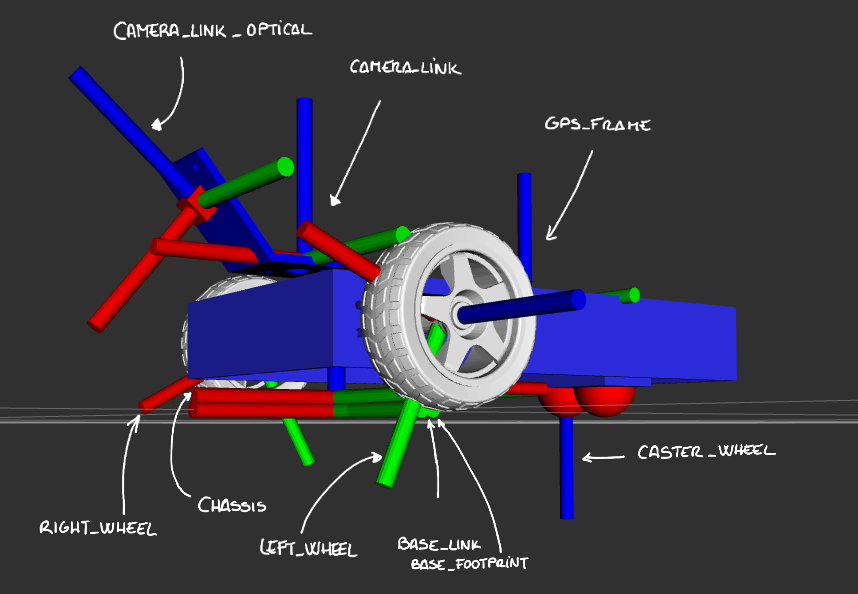
\includegraphics[width=12cm]{figs/cap6/links.png}
	\end{center}
	\caption{Sistemas de Coordenadas de PiBotJ}
	\label{fig:links}
\end{figure}\


\subsection{ROS 2 Control}

\subsubsection{Hardware Components/Interfaces}

 Tienen una comunicación directa con el hardware y existen tres tipos; en este caso, se decidió declarar todo el robot como un sistema para no limitar así el número de sensores y actuadores. 
 
 Si se quiere comprobar los hardware interfaces que tiene cualquier sistema, se puede hacer usando el siguiente comando: 
 \verb|ros2 control list_hardware_interfaces|

 
 Se puede ver que hay: (mostrar foto de output)
 
 %command interfaces
 %camera_joint/position [available] [claimed]
 %left_wheel_joint/velocity [available] [claimed]
 %right_wheel_joint/velocity [available] [claimed]
 %state interfaces
 %camera_joint/position
 %left_wheel_joint/position
 %left_wheel_joint/velocity
 %right_wheel_joint/position
 %right_wheel_joint/velocity
 
 Cada una de las command interfaces y state interfaces han sido definidas  para que el resource manager lo pueda usar gracias a la etiqueta <ros2\_control>. Dentro de esas etiquetas se asigna a cada joint el tipo de controller que se quiere usar. 
 
 Cada Hardware interface se configura usando un URDF. 
 
 
\subsubsection{Controllers}


Existen muchos tipos de controllers ya definidos, pero para este proyecto vamos a usar 2 tipos: diferencial y por posición. Para ello, es necesario definir sus parámetros a través de .yaml. 
En este caso, se llama my\_controllers.yaml. 



La rotación de la cámara (imagen y explicar cómo va)
ros2 Control  explicarlo


Creación de los topics que se quiera, la cámara por posición 

los topics que hay que lanzar 

he tenido que incluir el topic de la cámara, gps y de los motores

una vez se lanza el robot por primera vez puede fallar o tardar mucho, volver a lanzarlo


Explicar los topics que aparecen una vez ejecutado. 

Mostrar el video con el resultado final (rehacerlo)


\subsection{Robot State Publisher }

\subsection{Launcher}



\subsection{Ejemplo en funcionamiento}








\section{Vida real}

Configuración y comprobar que todas las partes funcionan

Explicar software creado para las dos versiones: teleoperado y autónomo

Modelo pin hole...

Shoelace method...

Capítulo 6: incluir lo de openvision paper\\









\section{Snippets}

Puede resultar interesante, para clarificar la descripción, mostrar fragmentos de código (o \textit{snippets}) ilustrativos. En el Código \ref{cod:codejemplo} vemos un ejemplo escrito en \texttt{C++}.

\begin{code}[h]
	\begin{lstlisting}[language=C++]
		void Memory::hypothesizeParallelograms () {
			for(it1 = this->controller->segmentMemory.begin(); it1++) {
				squareFound = false; it2 = it1; it2++;
				while ((it2 != this->controller->segmentMemory.end()) && (!squareFound)) {
					if (geometry::haveACommonVertex((*it1),(*it2),&square)) {
						dist1 = geometry::distanceBetweenPoints3D ((*it1).start, (*it1).end);
						dist2 = geometry::distanceBetweenPoints3D ((*it2).start, (*it2).end);
					}
					// [...]
				\end{lstlisting}
				\caption[Función para buscar elementos 3D en la imagen]{Función para buscar elementos 3D en la imagen}
				\label{cod:codejemplo}
			\end{code}
			
			En el Código \ref{cod:codejemplo2} vemos un ejemplo escrito en \texttt{Python}.
			
			\begin{code}[h]
				\begin{lstlisting}[language=Python]
					def mostrarValores():
					print (w1.get(), w2.get())
					
					master = Tk()
					w1 = Scale(master, from_=0, to=42)
					w1.pack()
					w2 = Scale(master, from_=0, to=200, orient=HORIZONTAL)
					w2.pack()
					Button(master, text='Show', command=mostrarValores).pack()
					
					mainloop()
				\end{lstlisting}
				\caption[Cómo usar un Slider]{Cómo usar un Slider}
				\label{cod:codejemplo2}
			\end{code}
			
			\section{Verbatim}
			
			Para mencionar identificadores usados en el código ---como nombres de funciones o variables--- en el texto, usa el entorno literal o verbatim \verb|hypothesizeParallelograms()|. También se puede usar este entorno para varias líneas, como se ve a continuación:
			
			\begin{verbatim}
				void Memory::hypothesizeParallelograms () {
					// add your code here
				}
			\end{verbatim}
			
			\section{Ecuaciones}
			
			Si necesitas insertar alguna ecuación, puedes hacerlo. Al igual que las figuras, no te olvides de referenciarlas. A continuación se exponen algunas ecuaciones de ejemplo: Ecuación \ref{ec:ec1} y Ecuación \ref{ec:ec2}.
			
			\begin{myequation}[h]
				\begin{equation}
					H = 1 - \frac{\sum_{i=0}^{N}\frac{(\frac{d_{j_s} + d_{j_e}}{2})}{N}}{M}
					\nonumber
					\label{ec:ec1}
				\end{equation}
				\caption[Ejemplo de ecuación con fracciones]{Ejemplo de ecuación con fracciones}
			\end{myequation} 
			
			\begin{myequation}[h]
				\begin{equation}
					v(entrada)= \left\{
					\begin{array}{lcc}
						0 & \mbox{if} & \epsilon_t < 0.1\\
						K_p\cdot{(T_{t}-T)} & \mbox{if}& 0.1 \leq \epsilon_t < M_t\\
						K_p \cdot M_t & \mbox{if}& M_t < \epsilon_t
					\end{array}
					\right.
					\label{ec:ec2}
				\end{equation}
				\caption[Ejemplo de ecuación con array y letras y símbolos especiales]{Ejemplo de ecuación con array y letras y símbolos especiales}
			\end{myequation}
			
			\section{Tablas o cuadros}
			
			Si necesitas insertar una tabla, hazlo dígnamente usando las propias tablas de \LaTeX, no usando pantallazos e insertándolas como figuras... En el Cuadro \ref{cuadro:ejemplo} vemos un ejemplo.
			
			\begin{table}[H]
				\begin{center}
					\begin{tabular}{|c|c|}
						\hline
						\textbf{Parámetros} & \textbf{Valores} \\
						\hline
						Tipo de sensor & Sony IMX219PQ[7] CMOS 8-Mpx \\
						Tamaño del sensor & 3.674 x 2.760 mm (1/4" format) \\
						Número de pixels & 3280 x 2464 (active pixels) \\
						Tamaño de pixel & 1.12 x 1.12 um \\
						Lente & f=3.04 mm, f/2.0 \\
						Ángulo de visión & 62.2 x 48.8 degrees \\
						Lente SLR equivalente & 29 mm \\
						\hline
					\end{tabular}
					\caption{Parámetros intrínsecos de la cámara}
					\label{cuadro:ejemplo}
				\end{center}
			\end{table}
			
			En los textos puedes poner palabras en \textit{cursiva}, para aquellas expresiones en sentido \textit{figurado}, palabras como \textit{robota}, que está fuera del diccionario castellano, o bien para resaltar palabras de una colección: \textit{(a)} es la primera letra del abecedario, \textit{(b)} es la segunda, etc.\\
			
			Al poner las dos líneas del anterior párrafo, este aparecerá separado del anterior. Si no las pongo, los párrafos aparecerán pegados. Sigue el criterio que consideres más oportuno.
			
			\section{Segunda sección}
			\label{sec:segundaseccion}
			
			No olvides incluir imágenes y referenciarlas, como la Figura \ref{fig:roomba}.
			
			\begin{figure} [h!]
				\begin{center}
					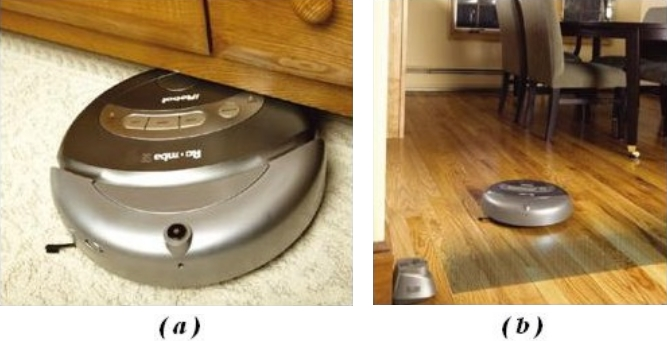
\includegraphics[width=8cm]{figs/roomba}
				\end{center}
				\caption{Robot aspirador Roomba de iRobot.}
				\label{fig:roomba}
			\end{figure}\
			
			Ni tampoco olvides de poner las URLs como notas al pie. Por ejemplo, si hablo de la Robocup\footnote{\url{http://www.robocup.org}}.
			
			\subsection{Números}
			\label{sec:subseccion}
			
			En lugar de tener secciones interminables, como la Sección \ref{sec:robotica}, divídelas en subsecciones.
			
			Para hablar de números, mételos en el entorno \textit{math} de \LaTeX, por ejemplo, $1.5Kg$. También puedes usar el símbolo del Euro como aquí: 1.500\euro.
			
			\subsection{Listas}
			
			Cuando describas una colección, usa \texttt{itemize} para ítems o \texttt{enumerate} para enumerados. Por ejemplo:
			
			\begin{itemize}
				\item \textit{Entorno de simulación.} Hemos usado dos entornos de simulación: uno en 3D y otro en 2D.
				\item \textit{Entornos reales.} Dentro del campus, hemos realizado experimentos en Biblioteca y en el edificio de Gestión.
			\end{itemize}\
			
			\begin{enumerate}
				\item Primer elemento de la colección.
				\item Segundo elemento de la colección.
			\end{enumerate}\
			
			\paragraph{Referencias bibliográficas}
			\label{sec:referencias}
			
			Cita, sobre todo en este capítulo, referencias bibliográficas que respalden tu argumento. Para citarlas basta con poner la instrucción \verb|\cite| con el identificador de la cita. Por ejemplo: libros como \cite{vega12e}, artículos como \cite{vega19b}, URLs como \cite{vega19a}, tesis como \cite{vega18b}, congresos como \cite{vega18a}, u otros trabajos fin de grado como \cite{vega08b}.
			
			Las referencias, con todo su contenido, están recogidas en el fichero \texttt{bibliografia.bib}. El contenido de estas referencias está en formato \texttt{BibTex}. Este formato se puede obtener en muchas ocasiones directamente, desde plataformas como \texttt{Google Scholar} u otros repositorios de recursos científicos.
			
			Existen numerosos estilos para reflejar una referencia bibliográfica. El estilo establecido por defecto en este documento es APA, que es uno de los estilos más comunes, pero lo puedes modificar en el archivo \texttt{memoria.tex}; concretamente, cambiando el campo \verb|apalike| a otro en la instrucción \verb|\bibliographystyle{apalike}|. 
			
			\
			
			\
			
			\
			
			Y, para terminar este capítulo, resume brevemente qué vas a contar en los siguientes.


\section{Corrector ortográfico}

Una vez tengas todo, no olvides pasar el corrector ortográfico de \LaTeX a todos tus ficheros \textit{.tex}. En \texttt{Windows}, el propio editor \texttt{TeXworks} incluye el corrector. En \texttt{Linux}, usa \texttt{aspell} ejecutando el siguiente comando en tu terminal:

\begin{verbatim}
aspell --lang=es --mode=tex check capitulo1.tex
\end{verbatim}
